\documentclass[1p]{elsarticle_modified}
%\bibliographystyle{elsarticle-num}

%\usepackage[colorlinks]{hyperref}
%\usepackage{abbrmath_seonhwa} %\Abb, \Ascr, \Acal ,\Abf, \Afrak
\usepackage{amsfonts}
\usepackage{amssymb}
\usepackage{amsmath}
\usepackage{amsthm}
\usepackage{scalefnt}
\usepackage{amsbsy}
\usepackage{kotex}
\usepackage{caption}
\usepackage{subfig}
\usepackage{color}
\usepackage{graphicx}
\usepackage{xcolor} %% white, black, red, green, blue, cyan, magenta, yellow
\usepackage{float}
\usepackage{setspace}
\usepackage{hyperref}

\usepackage{tikz}
\usetikzlibrary{arrows}

\usepackage{multirow}
\usepackage{array} % fixed length table
\usepackage{hhline}

%%%%%%%%%%%%%%%%%%%%%
\makeatletter
\renewcommand*\env@matrix[1][\arraystretch]{%
	\edef\arraystretch{#1}%
	\hskip -\arraycolsep
	\let\@ifnextchar\new@ifnextchar
	\array{*\c@MaxMatrixCols c}}
\makeatother %https://tex.stackexchange.com/questions/14071/how-can-i-increase-the-line-spacing-in-a-matrix
%%%%%%%%%%%%%%%

\usepackage[normalem]{ulem}

\newcommand{\msout}[1]{\ifmmode\text{\sout{\ensuremath{#1}}}\else\sout{#1}\fi}
%SOURCE: \msout is \stkout macro in https://tex.stackexchange.com/questions/20609/strikeout-in-math-mode

\newcommand{\cancel}[1]{
	\ifmmode
	{\color{red}\msout{#1}}
	\else
	{\color{red}\sout{#1}}
	\fi
}

\newcommand{\add}[1]{
	{\color{blue}\uwave{#1}}
}

\newcommand{\replace}[2]{
	\ifmmode
	{\color{red}\msout{#1}}{\color{blue}\uwave{#2}}
	\else
	{\color{red}\sout{#1}}{\color{blue}\uwave{#2}}
	\fi
}

\newcommand{\Sol}{\mathcal{S}} %segment
\newcommand{\D}{D} %diagram
\newcommand{\A}{\mathcal{A}} %arc


%%%%%%%%%%%%%%%%%%%%%%%%%%%%%5 test

\def\sl{\operatorname{\textup{SL}}(2,\Cbb)}
\def\psl{\operatorname{\textup{PSL}}(2,\Cbb)}
\def\quan{\mkern 1mu \triangleright \mkern 1mu}

\theoremstyle{definition}
\newtheorem{thm}{Theorem}[section]
\newtheorem{prop}[thm]{Proposition}
\newtheorem{lem}[thm]{Lemma}
\newtheorem{ques}[thm]{Question}
\newtheorem{cor}[thm]{Corollary}
\newtheorem{defn}[thm]{Definition}
\newtheorem{exam}[thm]{Example}
\newtheorem{rmk}[thm]{Remark}
\newtheorem{alg}[thm]{Algorithm}

\newcommand{\I}{\sqrt{-1}}
\begin{document}

%\begin{frontmatter}
%
%\title{Boundary parabolic representations of knots up to 8 crossings}
%
%%% Group authors per affiliation:
%\author{Yunhi Cho} 
%\address{Department of Mathematics, University of Seoul, Seoul, Korea}
%\ead{yhcho@uos.ac.kr}
%
%
%\author{Seonhwa Kim} %\fnref{s_kim}}
%\address{Center for Geometry and Physics, Institute for Basic Science, Pohang, 37673, Korea}
%\ead{ryeona17@ibs.re.kr}
%
%\author{Hyuk Kim}
%\address{Department of Mathematical Sciences, Seoul National University, Seoul 08826, Korea}
%\ead{hyukkim@snu.ac.kr}
%
%\author{Seokbeom Yoon}
%\address{Department of Mathematical Sciences, Seoul National University, Seoul, 08826,  Korea}
%\ead{sbyoon15@snu.ac.kr}
%
%\begin{abstract}
%We find all boundary parabolic representation of knots up to 8 crossings.
%
%\end{abstract}
%\begin{keyword}
%    \MSC[2010] 57M25 
%\end{keyword}
%
%\end{frontmatter}

%\linenumbers
%\tableofcontents
%
\newcommand\colored[1]{\textcolor{white}{\rule[-0.35ex]{0.8em}{1.4ex}}\kern-0.8em\color{red} #1}%
%\newcommand\colored[1]{\textcolor{white}{ #1}\kern-2.17ex	\textcolor{white}{ #1}\kern-1.81ex	\textcolor{white}{ #1}\kern-2.15ex\color{red}#1	}

{\Large $\underline{11a_{202}~(K11a_{202})}$}

\setlength{\tabcolsep}{10pt}
\renewcommand{\arraystretch}{1.6}
\vspace{1cm}\begin{tabular}{m{100pt}>{\centering\arraybackslash}m{274pt}}
\multirow{5}{120pt}{
	\centering
	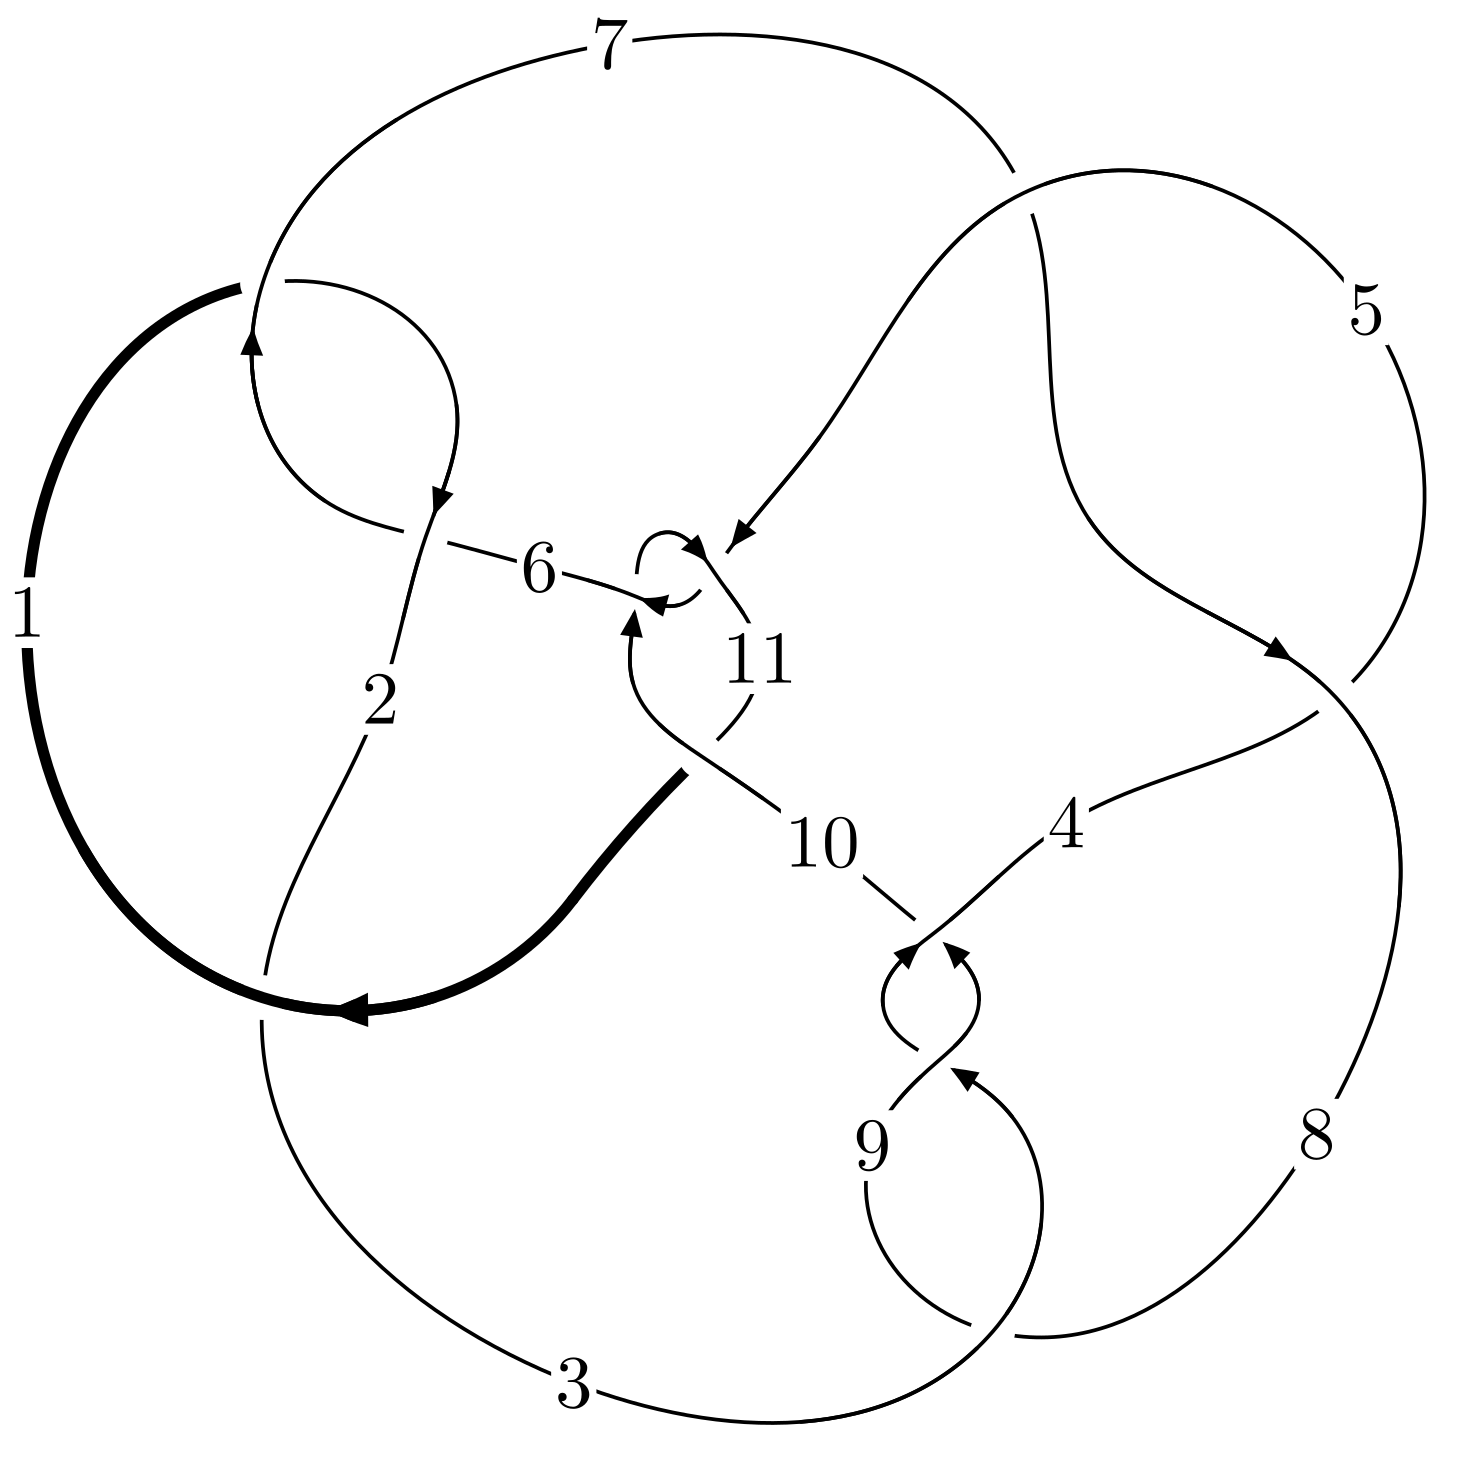
\includegraphics[width=112pt]{../../../GIT/diagram.site/Diagrams/png/451_11a_202.png}\\
\ \ \ A knot diagram\footnotemark}&
\allowdisplaybreaks
\textbf{Linearized knot diagam} \\
\cline{2-2}
 &
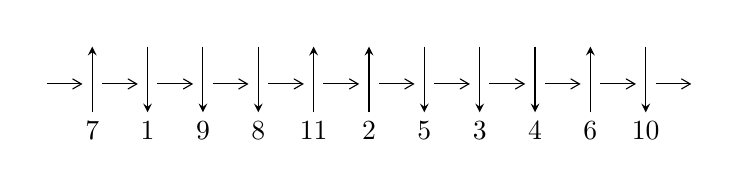
\begin{tikzpicture}[x=20pt, y=17pt]
	% nodes
	\node (C0) at (0, 0) {};
	\node (C1) at (1, 0) {};
	\node (C1U) at (1, +1) {};
	\node (C1D) at (1, -1) {7};

	\node (C2) at (2, 0) {};
	\node (C2U) at (2, +1) {};
	\node (C2D) at (2, -1) {1};

	\node (C3) at (3, 0) {};
	\node (C3U) at (3, +1) {};
	\node (C3D) at (3, -1) {9};

	\node (C4) at (4, 0) {};
	\node (C4U) at (4, +1) {};
	\node (C4D) at (4, -1) {8};

	\node (C5) at (5, 0) {};
	\node (C5U) at (5, +1) {};
	\node (C5D) at (5, -1) {11};

	\node (C6) at (6, 0) {};
	\node (C6U) at (6, +1) {};
	\node (C6D) at (6, -1) {2};

	\node (C7) at (7, 0) {};
	\node (C7U) at (7, +1) {};
	\node (C7D) at (7, -1) {5};

	\node (C8) at (8, 0) {};
	\node (C8U) at (8, +1) {};
	\node (C8D) at (8, -1) {3};

	\node (C9) at (9, 0) {};
	\node (C9U) at (9, +1) {};
	\node (C9D) at (9, -1) {4};

	\node (C10) at (10, 0) {};
	\node (C10U) at (10, +1) {};
	\node (C10D) at (10, -1) {6};

	\node (C11) at (11, 0) {};
	\node (C11U) at (11, +1) {};
	\node (C11D) at (11, -1) {10};
	\node (C12) at (12, 0) {};

	% arrows
	\draw[->,>={angle 60}]
	(C0) edge (C1) (C1) edge (C2) (C2) edge (C3) (C3) edge (C4) (C4) edge (C5) (C5) edge (C6) (C6) edge (C7) (C7) edge (C8) (C8) edge (C9) (C9) edge (C10) (C10) edge (C11) (C11) edge (C12) ;	\draw[->,>=stealth]
	(C1D) edge (C1U) (C2U) edge (C2D) (C3U) edge (C3D) (C4U) edge (C4D) (C5D) edge (C5U) (C6D) edge (C6U) (C7U) edge (C7D) (C8U) edge (C8D) (C9U) edge (C9D) (C10D) edge (C10U) (C11U) edge (C11D) ;
	\end{tikzpicture} \\
\hhline{~~} \\& 
\textbf{Solving Sequence} \\ \cline{2-2} 
 &
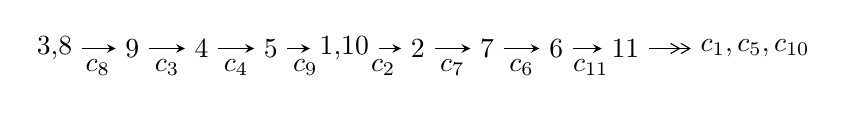
\begin{tikzpicture}[x=25pt, y=7pt]
	% node
	\node (A0) at (-1/8, 0) {3,8};
	\node (A1) at (1, 0) {9};
	\node (A2) at (2, 0) {4};
	\node (A3) at (3, 0) {5};
	\node (A4) at (65/16, 0) {1,10};
	\node (A5) at (41/8, 0) {2};
	\node (A6) at (49/8, 0) {7};
	\node (A7) at (57/8, 0) {6};
	\node (A8) at (65/8, 0) {11};
	\node (C1) at (1/2, -1) {$c_{8}$};
	\node (C2) at (3/2, -1) {$c_{3}$};
	\node (C3) at (5/2, -1) {$c_{4}$};
	\node (C4) at (7/2, -1) {$c_{9}$};
	\node (C5) at (37/8, -1) {$c_{2}$};
	\node (C6) at (45/8, -1) {$c_{7}$};
	\node (C7) at (53/8, -1) {$c_{6}$};
	\node (C8) at (61/8, -1) {$c_{11}$};
	\node (A9) at (10, 0) {$c_{1},c_{5},c_{10}$};

	% edge
	\draw[->,>=stealth]	
	(A0) edge (A1) (A1) edge (A2) (A2) edge (A3) (A3) edge (A4) (A4) edge (A5) (A5) edge (A6) (A6) edge (A7) (A7) edge (A8) ;
	\draw[->>,>={angle 60}]	
	(A8) edge (A9);
\end{tikzpicture} \\ 

\end{tabular} \\

\footnotetext{
The image of knot diagram is generated by the software ``\textbf{Draw programme}" developed by Andrew Bartholomew(\url{http://www.layer8.co.uk/maths/draw/index.htm\#Running-draw}), where we modified some parts for our purpose(\url{https://github.com/CATsTAILs/LinksPainter}).
}\phantom \\ \newline 
\centering \textbf{Ideals for irreducible components\footnotemark of $X_{\text{par}}$} 
 
\begin{align*}
I^u_{1}&=\langle 
3 u^{24}+5 u^{23}+\cdots+b+5,\;- u^{24}- u^{23}+\cdots+2 a-3,\;u^{25}+3 u^{24}+\cdots- u+2\rangle \\
I^u_{2}&=\langle 
- u^{17} a+u^{17}+\cdots- a+2,\;-2 u^{17} a+2 u^{17}+\cdots-3 a+5,\;u^{18}- u^{17}+\cdots+u-1\rangle \\
I^u_{3}&=\langle 
- u^5- u^4+2 u^3+2 u^2+b- u,\;u^5-3 u^3+a+2 u,\;u^6-3 u^4+2 u^2+1\rangle \\
\\
\end{align*}
\raggedright * 3 irreducible components of $\dim_{\mathbb{C}}=0$, with total 67 representations.\\
\footnotetext{All coefficients of polynomials are rational numbers. But the coefficients are sometimes approximated in decimal forms when there is not enough margin.}
\newpage
\renewcommand{\arraystretch}{1}
\centering \section*{I. $I^u_{1}= \langle 3 u^{24}+5 u^{23}+\cdots+b+5,\;- u^{24}- u^{23}+\cdots+2 a-3,\;u^{25}+3 u^{24}+\cdots- u+2 \rangle$}
\flushleft \textbf{(i) Arc colorings}\\
\begin{tabular}{m{7pt} m{180pt} m{7pt} m{180pt} }
\flushright $a_{3}=$&$\begin{pmatrix}0\\u\end{pmatrix}$ \\
\flushright $a_{8}=$&$\begin{pmatrix}1\\0\end{pmatrix}$ \\
\flushright $a_{9}=$&$\begin{pmatrix}1\\u^2\end{pmatrix}$ \\
\flushright $a_{4}=$&$\begin{pmatrix}- u\\- u^3+u\end{pmatrix}$ \\
\flushright $a_{5}=$&$\begin{pmatrix}u^3-2 u\\- u^3+u\end{pmatrix}$ \\
\flushright $a_{1}=$&$\begin{pmatrix}\frac{1}{2} u^{24}+\frac{1}{2} u^{23}+\cdots-\frac{5}{2} u+\frac{3}{2}\\-3 u^{24}-5 u^{23}+\cdots+7 u-5\end{pmatrix}$ \\
\flushright $a_{10}=$&$\begin{pmatrix}- u^2+1\\- u^4+2 u^2\end{pmatrix}$ \\
\flushright $a_{2}=$&$\begin{pmatrix}-\frac{1}{2} u^{24}-\frac{1}{2} u^{23}+\cdots+\frac{5}{2} u-\frac{3}{2}\\2 u^{24}+3 u^{23}+\cdots-3 u+3\end{pmatrix}$ \\
\flushright $a_{7}=$&$\begin{pmatrix}u^6-3 u^4+2 u^2+1\\- u^6+2 u^4- u^2\end{pmatrix}$ \\
\flushright $a_{6}=$&$\begin{pmatrix}\frac{3}{2} u^{24}+\frac{5}{2} u^{23}+\cdots-\frac{7}{2} u+\frac{5}{2}\\u^{24}+2 u^{23}+\cdots- u+1\end{pmatrix}$ \\
\flushright $a_{11}=$&$\begin{pmatrix}\frac{1}{2} u^{24}+\frac{1}{2} u^{23}+\cdots-\frac{3}{2} u+\frac{1}{2}\\-2 u^{24}-3 u^{23}+\cdots+4 u-3\end{pmatrix}$\\ \flushright $a_{11}=$&$\begin{pmatrix}\frac{1}{2} u^{24}+\frac{1}{2} u^{23}+\cdots-\frac{3}{2} u+\frac{1}{2}\\-2 u^{24}-3 u^{23}+\cdots+4 u-3\end{pmatrix}$\\&\end{tabular}
\flushleft \textbf{(ii) Obstruction class $= -1$}\\~\\
\flushleft \textbf{(iii) Cusp Shapes $= 12 u^{24}+22 u^{23}-96 u^{22}-160 u^{21}+354 u^{20}+456 u^{19}-774 u^{18}-512 u^{17}+1026 u^{16}-238 u^{15}-600 u^{14}+1204 u^{13}-430 u^{12}-908 u^{11}+980 u^{10}-316 u^9-372 u^8+598 u^7-292 u^6+150 u^4-100 u^3+72 u^2-28 u+18$}\\~\\
\newpage\renewcommand{\arraystretch}{1}
\flushleft \textbf{(iv) u-Polynomials at the component}\newline \\
\begin{tabular}{m{50pt}|m{274pt}}
Crossings & \hspace{64pt}u-Polynomials at each crossing \\
\hline $$\begin{aligned}c_{1},c_{5},c_{6}\\c_{10}\end{aligned}$$&$\begin{aligned}
&u^{25}+5 u^{23}+\cdots+5 u^2+1
\end{aligned}$\\
\hline $$\begin{aligned}c_{2},c_{11}\end{aligned}$$&$\begin{aligned}
&u^{25}+10 u^{24}+\cdots-10 u-1
\end{aligned}$\\
\hline $$\begin{aligned}c_{3},c_{8},c_{9}\end{aligned}$$&$\begin{aligned}
&u^{25}+3 u^{24}+\cdots- u+2
\end{aligned}$\\
\hline $$\begin{aligned}c_{4},c_{7}\end{aligned}$$&$\begin{aligned}
&u^{25}-9 u^{24}+\cdots+151 u-22
\end{aligned}$\\
\hline
\end{tabular}\\~\\
\newpage\renewcommand{\arraystretch}{1}
\flushleft \textbf{(v) Riley Polynomials at the component}\newline \\
\begin{tabular}{m{50pt}|m{274pt}}
Crossings & \hspace{64pt}Riley Polynomials at each crossing \\
\hline $$\begin{aligned}c_{1},c_{5},c_{6}\\c_{10}\end{aligned}$$&$\begin{aligned}
&y^{25}+10 y^{24}+\cdots-10 y-1
\end{aligned}$\\
\hline $$\begin{aligned}c_{2},c_{11}\end{aligned}$$&$\begin{aligned}
&y^{25}+18 y^{24}+\cdots+6 y-1
\end{aligned}$\\
\hline $$\begin{aligned}c_{3},c_{8},c_{9}\end{aligned}$$&$\begin{aligned}
&y^{25}-21 y^{24}+\cdots-19 y-4
\end{aligned}$\\
\hline $$\begin{aligned}c_{4},c_{7}\end{aligned}$$&$\begin{aligned}
&y^{25}+15 y^{24}+\cdots-563 y-484
\end{aligned}$\\
\hline
\end{tabular}\\~\\
\newpage\flushleft \textbf{(vi) Complex Volumes and Cusp Shapes}
$$\begin{array}{c|c|c}  
\text{Solutions to }I^u_{1}& \I (\text{vol} + \sqrt{-1}CS) & \text{Cusp shape}\\
 \hline 
\begin{aligned}
u &= \phantom{-}1.093170 + 0.381251 I \\
a &= \phantom{-}0.21753 - 1.41220 I \\
b &= \phantom{-}1.169580 - 0.560138 I\end{aligned}
 & \phantom{-}0.00199 + 6.23078 I & -4.13739 - 4.00981 I \\ \hline\begin{aligned}
u &= \phantom{-}1.093170 - 0.381251 I \\
a &= \phantom{-}0.21753 + 1.41220 I \\
b &= \phantom{-}1.169580 + 0.560138 I\end{aligned}
 & \phantom{-}0.00199 - 6.23078 I & -4.13739 + 4.00981 I \\ \hline\begin{aligned}
u &= \phantom{-}0.143356 + 0.825680 I \\
a &= \phantom{-}1.94580 - 0.73631 I \\
b &= -2.24518 + 0.45279 I\end{aligned}
 & \phantom{-}2.90521 - 10.60790 I & -1.48456 + 7.66724 I \\ \hline\begin{aligned}
u &= \phantom{-}0.143356 - 0.825680 I \\
a &= \phantom{-}1.94580 + 0.73631 I \\
b &= -2.24518 - 0.45279 I\end{aligned}
 & \phantom{-}2.90521 + 10.60790 I & -1.48456 - 7.66724 I \\ \hline\begin{aligned}
u &= \phantom{-}0.039360 + 0.824168 I \\
a &= -1.246860 + 0.327463 I \\
b &= \phantom{-}1.48748 + 0.14719 I\end{aligned}
 & \phantom{-}6.36489 + 0.77404 I & \phantom{-}3.16430 - 2.08441 I \\ \hline\begin{aligned}
u &= \phantom{-}0.039360 - 0.824168 I \\
a &= -1.246860 - 0.327463 I \\
b &= \phantom{-}1.48748 - 0.14719 I\end{aligned}
 & \phantom{-}6.36489 - 0.77404 I & \phantom{-}3.16430 + 2.08441 I \\ \hline\begin{aligned}
u &= -1.22317\phantom{ +0.000000I} \\
a &= \phantom{-}0.270576\phantom{ +0.000000I} \\
b &= -1.07819\phantom{ +0.000000I}\end{aligned}
 & -2.64205\phantom{ +0.000000I} & -1.56220\phantom{ +0.000000I} \\ \hline\begin{aligned}
u &= \phantom{-}0.607665 + 0.412689 I \\
a &= \phantom{-}1.67711 + 0.78738 I \\
b &= -0.641715 + 0.418679 I\end{aligned}
 & -1.35523 - 6.21788 I & -4.83403 + 8.18700 I \\ \hline\begin{aligned}
u &= \phantom{-}0.607665 - 0.412689 I \\
a &= \phantom{-}1.67711 - 0.78738 I \\
b &= -0.641715 - 0.418679 I\end{aligned}
 & -1.35523 + 6.21788 I & -4.83403 - 8.18700 I \\ \hline\begin{aligned}
u &= \phantom{-}1.226680 + 0.374932 I \\
a &= \phantom{-}0.111245 + 0.875220 I \\
b &= -0.651612 + 0.795102 I\end{aligned}
 & \phantom{-}2.70416 - 5.08779 I & -0.84739 + 5.77549 I\\
 \hline 
 \end{array}$$\newpage$$\begin{array}{c|c|c}  
\text{Solutions to }I^u_{1}& \I (\text{vol} + \sqrt{-1}CS) & \text{Cusp shape}\\
 \hline 
\begin{aligned}
u &= \phantom{-}1.226680 - 0.374932 I \\
a &= \phantom{-}0.111245 - 0.875220 I \\
b &= -0.651612 - 0.795102 I\end{aligned}
 & \phantom{-}2.70416 + 5.08779 I & -0.84739 - 5.77549 I \\ \hline\begin{aligned}
u &= \phantom{-}0.308716 + 0.611993 I \\
a &= -0.86404 - 1.36340 I \\
b &= \phantom{-}0.678982 + 0.816105 I\end{aligned}
 & -0.38145 + 2.56549 I & -2.38682 - 2.55463 I \\ \hline\begin{aligned}
u &= \phantom{-}0.308716 - 0.611993 I \\
a &= -0.86404 + 1.36340 I \\
b &= \phantom{-}0.678982 - 0.816105 I\end{aligned}
 & -0.38145 - 2.56549 I & -2.38682 + 2.55463 I \\ \hline\begin{aligned}
u &= -1.293350 + 0.365041 I \\
a &= \phantom{-}0.490950 - 0.568488 I \\
b &= -1.87489 - 0.82706 I\end{aligned}
 & \phantom{-}2.21088 + 3.50071 I & -0.821092 - 0.986963 I \\ \hline\begin{aligned}
u &= -1.293350 - 0.365041 I \\
a &= \phantom{-}0.490950 + 0.568488 I \\
b &= -1.87489 + 0.82706 I\end{aligned}
 & \phantom{-}2.21088 - 3.50071 I & -0.821092 + 0.986963 I \\ \hline\begin{aligned}
u &= \phantom{-}1.348970 + 0.191132 I \\
a &= \phantom{-}0.321151 + 0.095002 I \\
b &= \phantom{-}0.341623 + 0.269136 I\end{aligned}
 & -4.86135 - 3.43962 I & -5.00084 + 5.92088 I \\ \hline\begin{aligned}
u &= \phantom{-}1.348970 - 0.191132 I \\
a &= \phantom{-}0.321151 - 0.095002 I \\
b &= \phantom{-}0.341623 - 0.269136 I\end{aligned}
 & -4.86135 + 3.43962 I & -5.00084 - 5.92088 I \\ \hline\begin{aligned}
u &= -1.383170 + 0.239298 I \\
a &= -0.396095 - 0.636833 I \\
b &= -0.76363 + 1.37726 I\end{aligned}
 & -5.69008 + 0.51087 I & -7.53558 + 3.07532 I \\ \hline\begin{aligned}
u &= -1.383170 - 0.239298 I \\
a &= -0.396095 + 0.636833 I \\
b &= -0.76363 - 1.37726 I\end{aligned}
 & -5.69008 - 0.51087 I & -7.53558 - 3.07532 I \\ \hline\begin{aligned}
u &= -1.359100 + 0.357240 I \\
a &= -0.936093 + 0.861902 I \\
b &= \phantom{-}2.67364 + 1.62621 I\end{aligned}
 & -1.8285 + 14.8711 I & -5.98898 - 9.38448 I\\
 \hline 
 \end{array}$$\newpage$$\begin{array}{c|c|c}  
\text{Solutions to }I^u_{1}& \I (\text{vol} + \sqrt{-1}CS) & \text{Cusp shape}\\
 \hline 
\begin{aligned}
u &= -1.359100 - 0.357240 I \\
a &= -0.936093 - 0.861902 I \\
b &= \phantom{-}2.67364 - 1.62621 I\end{aligned}
 & -1.8285 - 14.8711 I & -5.98898 + 9.38448 I \\ \hline\begin{aligned}
u &= -1.41996 + 0.07613 I \\
a &= -0.691382 + 0.771202 I \\
b &= \phantom{-}1.38435 - 0.56025 I\end{aligned}
 & -7.78094 + 7.61728 I & -9.88218 - 7.10707 I \\ \hline\begin{aligned}
u &= -1.41996 - 0.07613 I \\
a &= -0.691382 - 0.771202 I \\
b &= \phantom{-}1.38435 + 0.56025 I\end{aligned}
 & -7.78094 - 7.61728 I & -9.88218 + 7.10707 I \\ \hline\begin{aligned}
u &= -0.200761 + 0.437718 I \\
a &= -0.514596 - 0.165982 I \\
b &= -0.019513 + 0.393038 I\end{aligned}
 & -0.015654 + 1.044500 I & -0.46434 - 6.95411 I \\ \hline\begin{aligned}
u &= -0.200761 - 0.437718 I \\
a &= -0.514596 + 0.165982 I \\
b &= -0.019513 - 0.393038 I\end{aligned}
 & -0.015654 - 1.044500 I & -0.46434 + 6.95411 I\\
 \hline 
 \end{array}$$\newpage\newpage\renewcommand{\arraystretch}{1}
\centering \section*{II. $I^u_{2}= \langle - u^{17} a+u^{17}+\cdots- a+2,\;-2 u^{17} a+2 u^{17}+\cdots-3 a+5,\;u^{18}- u^{17}+\cdots+u-1 \rangle$}
\flushleft \textbf{(i) Arc colorings}\\
\begin{tabular}{m{7pt} m{180pt} m{7pt} m{180pt} }
\flushright $a_{3}=$&$\begin{pmatrix}0\\u\end{pmatrix}$ \\
\flushright $a_{8}=$&$\begin{pmatrix}1\\0\end{pmatrix}$ \\
\flushright $a_{9}=$&$\begin{pmatrix}1\\u^2\end{pmatrix}$ \\
\flushright $a_{4}=$&$\begin{pmatrix}- u\\- u^3+u\end{pmatrix}$ \\
\flushright $a_{5}=$&$\begin{pmatrix}u^3-2 u\\- u^3+u\end{pmatrix}$ \\
\flushright $a_{1}=$&$\begin{pmatrix}a\\u^{17} a- u^{17}+\cdots+a-2\end{pmatrix}$ \\
\flushright $a_{10}=$&$\begin{pmatrix}- u^2+1\\- u^4+2 u^2\end{pmatrix}$ \\
\flushright $a_{2}=$&$\begin{pmatrix}u^{17} a- u^{17}+\cdots+2 a-2\\u^{17} a- u^{17}+\cdots+a-2\end{pmatrix}$ \\
\flushright $a_{7}=$&$\begin{pmatrix}u^6-3 u^4+2 u^2+1\\- u^6+2 u^4- u^2\end{pmatrix}$ \\
\flushright $a_{6}=$&$\begin{pmatrix}u^{17} a-2 u^{17}+\cdots+2 a-5\\- u^{17}+7 u^{15}+\cdots- a u+u\end{pmatrix}$ \\
\flushright $a_{11}=$&$\begin{pmatrix}u^{16}-7 u^{14}+\cdots+a-1\\u^{17} a- u^{17}+\cdots+a-2\end{pmatrix}$\\ \flushright $a_{11}=$&$\begin{pmatrix}u^{16}-7 u^{14}+\cdots+a-1\\u^{17} a- u^{17}+\cdots+a-2\end{pmatrix}$\\&\end{tabular}
\flushleft \textbf{(ii) Obstruction class $= -1$}\\~\\
\flushleft \textbf{(iii) Cusp Shapes $= 4 u^{15}-24 u^{13}-4 u^{12}+56 u^{11}+20 u^{10}-52 u^9-36 u^8-8 u^7+20 u^6+44 u^5+12 u^4-12 u^3-12 u^2-12 u-6$}\\~\\
\newpage\renewcommand{\arraystretch}{1}
\flushleft \textbf{(iv) u-Polynomials at the component}\newline \\
\begin{tabular}{m{50pt}|m{274pt}}
Crossings & \hspace{64pt}u-Polynomials at each crossing \\
\hline $$\begin{aligned}c_{1},c_{5},c_{6}\\c_{10}\end{aligned}$$&$\begin{aligned}
&u^{36}+u^{35}+\cdots+2 u+5
\end{aligned}$\\
\hline $$\begin{aligned}c_{2},c_{11}\end{aligned}$$&$\begin{aligned}
&u^{36}+19 u^{35}+\cdots+136 u+25
\end{aligned}$\\
\hline $$\begin{aligned}c_{3},c_{8},c_{9}\end{aligned}$$&$\begin{aligned}
&(u^{18}- u^{17}+\cdots+u-1)^{2}
\end{aligned}$\\
\hline $$\begin{aligned}c_{4},c_{7}\end{aligned}$$&$\begin{aligned}
&(u^{18}+3 u^{17}+\cdots+3 u+3)^{2}
\end{aligned}$\\
\hline
\end{tabular}\\~\\
\newpage\renewcommand{\arraystretch}{1}
\flushleft \textbf{(v) Riley Polynomials at the component}\newline \\
\begin{tabular}{m{50pt}|m{274pt}}
Crossings & \hspace{64pt}Riley Polynomials at each crossing \\
\hline $$\begin{aligned}c_{1},c_{5},c_{6}\\c_{10}\end{aligned}$$&$\begin{aligned}
&y^{36}+19 y^{35}+\cdots+136 y+25
\end{aligned}$\\
\hline $$\begin{aligned}c_{2},c_{11}\end{aligned}$$&$\begin{aligned}
&y^{36}-5 y^{35}+\cdots+4204 y+625
\end{aligned}$\\
\hline $$\begin{aligned}c_{3},c_{8},c_{9}\end{aligned}$$&$\begin{aligned}
&(y^{18}-15 y^{17}+\cdots-7 y+1)^{2}
\end{aligned}$\\
\hline $$\begin{aligned}c_{4},c_{7}\end{aligned}$$&$\begin{aligned}
&(y^{18}+13 y^{17}+\cdots-75 y+9)^{2}
\end{aligned}$\\
\hline
\end{tabular}\\~\\
\newpage\flushleft \textbf{(vi) Complex Volumes and Cusp Shapes}
$$\begin{array}{c|c|c}  
\text{Solutions to }I^u_{2}& \I (\text{vol} + \sqrt{-1}CS) & \text{Cusp shape}\\
 \hline 
\begin{aligned}
u &= -0.099390 + 0.822674 I \\
a &= \phantom{-}1.010160 + 0.659261 I \\
b &= -1.204720 - 0.060446 I\end{aligned}
 & \phantom{-}5.09742 + 4.87394 I & \phantom{-}1.52680 - 3.60136 I \\ \hline\begin{aligned}
u &= -0.099390 + 0.822674 I \\
a &= -1.77185 - 0.50072 I \\
b &= \phantom{-}2.12693 + 0.43784 I\end{aligned}
 & \phantom{-}5.09742 + 4.87394 I & \phantom{-}1.52680 - 3.60136 I \\ \hline\begin{aligned}
u &= -0.099390 - 0.822674 I \\
a &= \phantom{-}1.010160 - 0.659261 I \\
b &= -1.204720 + 0.060446 I\end{aligned}
 & \phantom{-}5.09742 - 4.87394 I & \phantom{-}1.52680 + 3.60136 I \\ \hline\begin{aligned}
u &= -0.099390 - 0.822674 I \\
a &= -1.77185 + 0.50072 I \\
b &= \phantom{-}2.12693 - 0.43784 I\end{aligned}
 & \phantom{-}5.09742 - 4.87394 I & \phantom{-}1.52680 + 3.60136 I \\ \hline\begin{aligned}
u &= -1.160030 + 0.371279 I \\
a &= -0.005598 - 1.165270 I \\
b &= -1.48494 - 0.71912 I\end{aligned}
 & \phantom{-}1.85527 - 0.55896 I & -1.51114 - 0.25710 I \\ \hline\begin{aligned}
u &= -1.160030 + 0.371279 I \\
a &= \phantom{-}0.193687 + 0.796364 I \\
b &= \phantom{-}0.184198 + 0.414383 I\end{aligned}
 & \phantom{-}1.85527 - 0.55896 I & -1.51114 - 0.25710 I \\ \hline\begin{aligned}
u &= -1.160030 - 0.371279 I \\
a &= -0.005598 + 1.165270 I \\
b &= -1.48494 + 0.71912 I\end{aligned}
 & \phantom{-}1.85527 + 0.55896 I & -1.51114 + 0.25710 I \\ \hline\begin{aligned}
u &= -1.160030 - 0.371279 I \\
a &= \phantom{-}0.193687 - 0.796364 I \\
b &= \phantom{-}0.184198 - 0.414383 I\end{aligned}
 & \phantom{-}1.85527 + 0.55896 I & -1.51114 + 0.25710 I \\ \hline\begin{aligned}
u &= \phantom{-}0.064741 + 0.739221 I \\
a &= \phantom{-}1.151170 - 0.650197 I \\
b &= -2.00838 + 0.88685 I\end{aligned}
 & -0.86368 - 1.88569 I & -1.68331 + 3.99357 I \\ \hline\begin{aligned}
u &= \phantom{-}0.064741 + 0.739221 I \\
a &= -0.25126 - 2.22448 I \\
b &= \phantom{-}0.20114 + 1.41506 I\end{aligned}
 & -0.86368 - 1.88569 I & -1.68331 + 3.99357 I\\
 \hline 
 \end{array}$$\newpage$$\begin{array}{c|c|c}  
\text{Solutions to }I^u_{2}& \I (\text{vol} + \sqrt{-1}CS) & \text{Cusp shape}\\
 \hline 
\begin{aligned}
u &= \phantom{-}0.064741 - 0.739221 I \\
a &= \phantom{-}1.151170 + 0.650197 I \\
b &= -2.00838 - 0.88685 I\end{aligned}
 & -0.86368 + 1.88569 I & -1.68331 - 3.99357 I \\ \hline\begin{aligned}
u &= \phantom{-}0.064741 - 0.739221 I \\
a &= -0.25126 + 2.22448 I \\
b &= \phantom{-}0.20114 - 1.41506 I\end{aligned}
 & -0.86368 + 1.88569 I & -1.68331 - 3.99357 I \\ \hline\begin{aligned}
u &= \phantom{-}1.232890 + 0.279362 I \\
a &= \phantom{-}1.254980 - 0.181881 I \\
b &= -0.38174 + 1.40962 I\end{aligned}
 & -4.41864 - 1.78695 I & -5.23943 - 0.02251 I \\ \hline\begin{aligned}
u &= \phantom{-}1.232890 + 0.279362 I \\
a &= \phantom{-}0.162452 - 0.553286 I \\
b &= \phantom{-}2.09907 - 1.16052 I\end{aligned}
 & -4.41864 - 1.78695 I & -5.23943 - 0.02251 I \\ \hline\begin{aligned}
u &= \phantom{-}1.232890 - 0.279362 I \\
a &= \phantom{-}1.254980 + 0.181881 I \\
b &= -0.38174 - 1.40962 I\end{aligned}
 & -4.41864 + 1.78695 I & -5.23943 + 0.02251 I \\ \hline\begin{aligned}
u &= \phantom{-}1.232890 - 0.279362 I \\
a &= \phantom{-}0.162452 + 0.553286 I \\
b &= \phantom{-}2.09907 + 1.16052 I\end{aligned}
 & -4.41864 + 1.78695 I & -5.23943 + 0.02251 I \\ \hline\begin{aligned}
u &= -1.34147\phantom{ +0.000000I} \\
a &= -0.909316 + 0.569963 I \\
b &= \phantom{-}1.93594 + 0.69913 I\end{aligned}
 & -9.12242\phantom{ +0.000000I} & -12.3720\phantom{ +0.000000I} \\ \hline\begin{aligned}
u &= -1.34147\phantom{ +0.000000I} \\
a &= -0.909316 - 0.569963 I \\
b &= \phantom{-}1.93594 - 0.69913 I\end{aligned}
 & -9.12242\phantom{ +0.000000I} & -12.3720\phantom{ +0.000000I} \\ \hline\begin{aligned}
u &= -1.311620 + 0.317206 I \\
a &= -0.639151 + 0.570901 I \\
b &= \phantom{-}1.49141 + 2.61785 I\end{aligned}
 & -5.17867 + 5.71427 I & -7.06596 - 6.05983 I \\ \hline\begin{aligned}
u &= -1.311620 + 0.317206 I \\
a &= -1.126620 - 0.630098 I \\
b &= \phantom{-}0.05295 + 1.74084 I\end{aligned}
 & -5.17867 + 5.71427 I & -7.06596 - 6.05983 I\\
 \hline 
 \end{array}$$\newpage$$\begin{array}{c|c|c}  
\text{Solutions to }I^u_{2}& \I (\text{vol} + \sqrt{-1}CS) & \text{Cusp shape}\\
 \hline 
\begin{aligned}
u &= -1.311620 - 0.317206 I \\
a &= -0.639151 - 0.570901 I \\
b &= \phantom{-}1.49141 - 2.61785 I\end{aligned}
 & -5.17867 - 5.71427 I & -7.06596 + 6.05983 I \\ \hline\begin{aligned}
u &= -1.311620 - 0.317206 I \\
a &= -1.126620 + 0.630098 I \\
b &= \phantom{-}0.05295 - 1.74084 I\end{aligned}
 & -5.17867 - 5.71427 I & -7.06596 + 6.05983 I \\ \hline\begin{aligned}
u &= \phantom{-}1.354280 + 0.099636 I \\
a &= \phantom{-}0.688151 + 0.512494 I \\
b &= -0.934430 + 0.141070 I\end{aligned}
 & -5.44315 - 3.22673 I & -7.05526 + 3.62956 I \\ \hline\begin{aligned}
u &= \phantom{-}1.354280 + 0.099636 I \\
a &= -0.240178 - 0.159767 I \\
b &= \phantom{-}1.40470 + 0.41204 I\end{aligned}
 & -5.44315 - 3.22673 I & -7.05526 + 3.62956 I \\ \hline\begin{aligned}
u &= \phantom{-}1.354280 - 0.099636 I \\
a &= \phantom{-}0.688151 - 0.512494 I \\
b &= -0.934430 - 0.141070 I\end{aligned}
 & -5.44315 + 3.22673 I & -7.05526 - 3.62956 I \\ \hline\begin{aligned}
u &= \phantom{-}1.354280 - 0.099636 I \\
a &= -0.240178 + 0.159767 I \\
b &= \phantom{-}1.40470 - 0.41204 I\end{aligned}
 & -5.44315 + 3.22673 I & -7.05526 - 3.62956 I \\ \hline\begin{aligned}
u &= \phantom{-}1.333560 + 0.360812 I \\
a &= \phantom{-}0.761590 + 0.869340 I \\
b &= -2.17073 + 1.60538 I\end{aligned}
 & \phantom{-}0.60037 - 9.13509 I & -2.98695 + 5.86478 I \\ \hline\begin{aligned}
u &= \phantom{-}1.333560 + 0.360812 I \\
a &= -0.633768 - 0.345440 I \\
b &= \phantom{-}1.83682 - 0.93179 I\end{aligned}
 & \phantom{-}0.60037 - 9.13509 I & -2.98695 + 5.86478 I \\ \hline\begin{aligned}
u &= \phantom{-}1.333560 - 0.360812 I \\
a &= \phantom{-}0.761590 - 0.869340 I \\
b &= -2.17073 - 1.60538 I\end{aligned}
 & \phantom{-}0.60037 + 9.13509 I & -2.98695 - 5.86478 I \\ \hline\begin{aligned}
u &= \phantom{-}1.333560 - 0.360812 I \\
a &= -0.633768 + 0.345440 I \\
b &= \phantom{-}1.83682 + 0.93179 I\end{aligned}
 & \phantom{-}0.60037 + 9.13509 I & -2.98695 - 5.86478 I\\
 \hline 
 \end{array}$$\newpage$$\begin{array}{c|c|c}  
\text{Solutions to }I^u_{2}& \I (\text{vol} + \sqrt{-1}CS) & \text{Cusp shape}\\
 \hline 
\begin{aligned}
u &= -0.424636 + 0.422216 I \\
a &= \phantom{-}0.754958 - 0.611235 I \\
b &= -0.588599 + 0.366257 I\end{aligned}
 & \phantom{-}0.06375 + 1.57187 I & -1.80878 - 4.22070 I \\ \hline\begin{aligned}
u &= -0.424636 + 0.422216 I \\
a &= -1.36523 + 0.46965 I \\
b &= \phantom{-}0.340053 + 0.339838 I\end{aligned}
 & \phantom{-}0.06375 + 1.57187 I & -1.80878 - 4.22070 I \\ \hline\begin{aligned}
u &= -0.424636 - 0.422216 I \\
a &= \phantom{-}0.754958 + 0.611235 I \\
b &= -0.588599 - 0.366257 I\end{aligned}
 & \phantom{-}0.06375 - 1.57187 I & -1.80878 + 4.22070 I \\ \hline\begin{aligned}
u &= -0.424636 - 0.422216 I \\
a &= -1.36523 - 0.46965 I \\
b &= \phantom{-}0.340053 - 0.339838 I\end{aligned}
 & \phantom{-}0.06375 - 1.57187 I & -1.80878 + 4.22070 I \\ \hline\begin{aligned}
u &= \phantom{-}0.361873\phantom{ +0.000000I} \\
a &= \phantom{-}2.96583 + 1.11433 I \\
b &= -0.399690 + 0.777849 I\end{aligned}
 & -3.91179\phantom{ +0.000000I} & -11.9800\phantom{ +0.000000I} \\ \hline\begin{aligned}
u &= \phantom{-}0.361873\phantom{ +0.000000I} \\
a &= \phantom{-}2.96583 - 1.11433 I \\
b &= -0.399690 - 0.777849 I\end{aligned}
 & -3.91179\phantom{ +0.000000I} & -11.9800\phantom{ +0.000000I}\\
 \hline 
 \end{array}$$\newpage\newpage\renewcommand{\arraystretch}{1}
\centering \section*{III. $I^u_{3}= \langle - u^5- u^4+2 u^3+2 u^2+b- u,\;u^5-3 u^3+a+2 u,\;u^6-3 u^4+2 u^2+1 \rangle$}
\flushleft \textbf{(i) Arc colorings}\\
\begin{tabular}{m{7pt} m{180pt} m{7pt} m{180pt} }
\flushright $a_{3}=$&$\begin{pmatrix}0\\u\end{pmatrix}$ \\
\flushright $a_{8}=$&$\begin{pmatrix}1\\0\end{pmatrix}$ \\
\flushright $a_{9}=$&$\begin{pmatrix}1\\u^2\end{pmatrix}$ \\
\flushright $a_{4}=$&$\begin{pmatrix}- u\\- u^3+u\end{pmatrix}$ \\
\flushright $a_{5}=$&$\begin{pmatrix}u^3-2 u\\- u^3+u\end{pmatrix}$ \\
\flushright $a_{1}=$&$\begin{pmatrix}- u^5+3 u^3-2 u\\u^5+u^4-2 u^3-2 u^2+u\end{pmatrix}$ \\
\flushright $a_{10}=$&$\begin{pmatrix}- u^2+1\\- u^4+2 u^2\end{pmatrix}$ \\
\flushright $a_{2}=$&$\begin{pmatrix}- u^5+3 u^3-2 u\\u^5+u^4-2 u^3-2 u^2+2 u\end{pmatrix}$ \\
\flushright $a_{7}=$&$\begin{pmatrix}0\\- u^4+u^2+1\end{pmatrix}$ \\
\flushright $a_{6}=$&$\begin{pmatrix}u^4-2 u^2+1\\- u^3+u-1\end{pmatrix}$ \\
\flushright $a_{11}=$&$\begin{pmatrix}- u^5+3 u^3- u^2-2 u+1\\u^5-2 u^3+u\end{pmatrix}$\\ \flushright $a_{11}=$&$\begin{pmatrix}- u^5+3 u^3- u^2-2 u+1\\u^5-2 u^3+u\end{pmatrix}$\\&\end{tabular}
\flushleft \textbf{(ii) Obstruction class $= 1$}\\~\\
\flushleft \textbf{(iii) Cusp Shapes $= 4 u^4-8 u^2-8$}\\~\\
\newpage\renewcommand{\arraystretch}{1}
\flushleft \textbf{(iv) u-Polynomials at the component}\newline \\
\begin{tabular}{m{50pt}|m{274pt}}
Crossings & \hspace{64pt}u-Polynomials at each crossing \\
\hline $$\begin{aligned}c_{1},c_{5},c_{6}\\c_{10}\end{aligned}$$&$\begin{aligned}
&(u^2+1)^3
\end{aligned}$\\
\hline $$\begin{aligned}c_{2},c_{11}\end{aligned}$$&$\begin{aligned}
&(u+1)^6
\end{aligned}$\\
\hline $$\begin{aligned}c_{3},c_{8},c_{9}\end{aligned}$$&$\begin{aligned}
&u^6-3 u^4+2 u^2+1
\end{aligned}$\\
\hline $$\begin{aligned}c_{4},c_{7}\end{aligned}$$&$\begin{aligned}
&u^6+u^4+2 u^2+1
\end{aligned}$\\
\hline
\end{tabular}\\~\\
\newpage\renewcommand{\arraystretch}{1}
\flushleft \textbf{(v) Riley Polynomials at the component}\newline \\
\begin{tabular}{m{50pt}|m{274pt}}
Crossings & \hspace{64pt}Riley Polynomials at each crossing \\
\hline $$\begin{aligned}c_{1},c_{5},c_{6}\\c_{10}\end{aligned}$$&$\begin{aligned}
&(y+1)^6
\end{aligned}$\\
\hline $$\begin{aligned}c_{2},c_{11}\end{aligned}$$&$\begin{aligned}
&(y-1)^6
\end{aligned}$\\
\hline $$\begin{aligned}c_{3},c_{8},c_{9}\end{aligned}$$&$\begin{aligned}
&(y^3-3 y^2+2 y+1)^2
\end{aligned}$\\
\hline $$\begin{aligned}c_{4},c_{7}\end{aligned}$$&$\begin{aligned}
&(y^3+y^2+2 y+1)^2
\end{aligned}$\\
\hline
\end{tabular}\\~\\
\newpage\flushleft \textbf{(vi) Complex Volumes and Cusp Shapes}
$$\begin{array}{c|c|c}  
\text{Solutions to }I^u_{3}& \I (\text{vol} + \sqrt{-1}CS) & \text{Cusp shape}\\
 \hline 
\begin{aligned}
u &= \phantom{-}1.307140 + 0.215080 I \\
a &= \phantom{-}0.744862 - 0.122561 I \\
b &= -0.87744 + 1.74486 I\end{aligned}
 & -6.31400 - 2.82812 I & -11.50976 + 2.97945 I \\ \hline\begin{aligned}
u &= \phantom{-}1.307140 - 0.215080 I \\
a &= \phantom{-}0.744862 + 0.122561 I \\
b &= -0.87744 - 1.74486 I\end{aligned}
 & -6.31400 + 2.82812 I & -11.50976 - 2.97945 I \\ \hline\begin{aligned}
u &= -1.307140 + 0.215080 I \\
a &= -0.744862 - 0.122561 I \\
b &= -0.877439 + 0.255138 I\end{aligned}
 & -6.31400 + 2.82812 I & -11.50976 - 2.97945 I \\ \hline\begin{aligned}
u &= -1.307140 - 0.215080 I \\
a &= -0.744862 + 0.122561 I \\
b &= -0.877439 - 0.255138 I\end{aligned}
 & -6.31400 - 2.82812 I & -11.50976 + 2.97945 I \\ \hline\begin{aligned}
u &= \phantom{-0.000000 -}0.569840 I \\
a &= \phantom{-0.000000 } -1.75488 I \\
b &= \phantom{-}0.754878 + 1.000000 I\end{aligned}
 & -2.17641\phantom{ +0.000000I} & -4.98050\phantom{ +0.000000I} \\ \hline\begin{aligned}
u &= \phantom{-0.000000 } -0.569840 I \\
a &= \phantom{-0.000000 -}1.75488 I \\
b &= \phantom{-}0.754878 - 1.000000 I\end{aligned}
 & -2.17641\phantom{ +0.000000I} & -4.98050\phantom{ +0.000000I}\\
 \hline 
 \end{array}$$\newpage
\newpage\renewcommand{\arraystretch}{1}
\centering \section*{ IV. u-Polynomials}
\begin{tabular}{m{50pt}|m{274pt}}
Crossings & \hspace{64pt}u-Polynomials at each crossing \\
\hline $$\begin{aligned}c_{1},c_{5},c_{6}\\c_{10}\end{aligned}$$&$\begin{aligned}
&((u^2+1)^3)(u^{25}+5 u^{23}+\cdots+5 u^2+1)(u^{36}+u^{35}+\cdots+2 u+5)
\end{aligned}$\\
\hline $$\begin{aligned}c_{2},c_{11}\end{aligned}$$&$\begin{aligned}
&((u+1)^6)(u^{25}+10 u^{24}+\cdots-10 u-1)(u^{36}+19 u^{35}+\cdots+136 u+25)
\end{aligned}$\\
\hline $$\begin{aligned}c_{3},c_{8},c_{9}\end{aligned}$$&$\begin{aligned}
&(u^6-3 u^4+2 u^2+1)(u^{18}- u^{17}+\cdots+u-1)^{2}(u^{25}+3 u^{24}+\cdots- u+2)
\end{aligned}$\\
\hline $$\begin{aligned}c_{4},c_{7}\end{aligned}$$&$\begin{aligned}
&(u^6+u^4+2 u^2+1)(u^{18}+3 u^{17}+\cdots+3 u+3)^{2}\\
&\cdot(u^{25}-9 u^{24}+\cdots+151 u-22)
\end{aligned}$\\
\hline
\end{tabular}\newpage\renewcommand{\arraystretch}{1}
\centering \section*{ V. Riley Polynomials}
\begin{tabular}{m{50pt}|m{274pt}}
Crossings & \hspace{64pt}Riley Polynomials at each crossing \\
\hline $$\begin{aligned}c_{1},c_{5},c_{6}\\c_{10}\end{aligned}$$&$\begin{aligned}
&((y+1)^6)(y^{25}+10 y^{24}+\cdots-10 y-1)(y^{36}+19 y^{35}+\cdots+136 y+25)
\end{aligned}$\\
\hline $$\begin{aligned}c_{2},c_{11}\end{aligned}$$&$\begin{aligned}
&((y-1)^6)(y^{25}+18 y^{24}+\cdots+6 y-1)(y^{36}-5 y^{35}+\cdots+4204 y+625)
\end{aligned}$\\
\hline $$\begin{aligned}c_{3},c_{8},c_{9}\end{aligned}$$&$\begin{aligned}
&((y^3-3 y^2+2 y+1)^2)(y^{18}-15 y^{17}+\cdots-7 y+1)^{2}\\
&\cdot(y^{25}-21 y^{24}+\cdots-19 y-4)
\end{aligned}$\\
\hline $$\begin{aligned}c_{4},c_{7}\end{aligned}$$&$\begin{aligned}
&((y^3+y^2+2 y+1)^2)(y^{18}+13 y^{17}+\cdots-75 y+9)^{2}\\
&\cdot(y^{25}+15 y^{24}+\cdots-563 y-484)
\end{aligned}$\\
\hline
\end{tabular}
\vskip 2pc
\end{document}